
\documentclass{beamer}


\mode<presentation>
{
  \usetheme{CambridgeUS}
	\usecolortheme{beaver}
  % or ...

  \setbeamercovered{transparent}
  % or whatever (possibly just delete it)
}


\usepackage{xeCJK}
\usepackage[english]{babel}
\usepackage[utf8]{inputenc}
\usepackage{times}
\usepackage[T1]{fontenc}
\usepackage{hyperref}
\usepackage{pifont}
\usepackage{bibentry}
\usepackage{verbatim}
\usepackage{color}
\usepackage{tikz}
\usetikzlibrary{arrows.meta, positioning}
\newcommand{\cmark}{\ding{51}}%
\newcommand{\xmark}{\ding{55}}%
\setCJKmainfont{WenQuanYi Micro Hei}
\renewcommand{\raggedright}{\leftskip=0pt \rightskip=0pt plus 0cm}
\raggedright

\let\oldfootnotesize\footnotesize
\renewcommand*{\footnotesize}{\oldfootnotesize\tiny}

\usepackage{listings}
\usepackage{xcolor}

\lstset{
  language=C++,
  basicstyle=\ttfamily\tiny,
  keywordstyle=\color{blue},
  commentstyle=\color{gray},
  stringstyle=\color{red},
  breaklines=true,
  columns=fullflexible,
}

\title[开源软件基础] 
{开源软件基础}
\subtitle{编译器测试}

\author[Zhilei Ren] 
{Zhilei Ren}

\institute[OSCAR Team] % (optional, but mostly needed)
{
\\
\includegraphics[width=0.2\textwidth]{../../utils/logo.jpg}\\
OSCAR Team, School of Software, 
Dalian University of Technology
}


\subject{Open source}



\pgfdeclareimage[height=0.5cm]{university-logo}{../../utils/logo.jpg}
\logo{\pgfuseimage{university-logo}}



% Delete this, if you do not want the table of contents to pop up at
% the beginning of each subsection:
\AtBeginSubsection[]
{
  \begin{frame}<beamer>{Outline}
    \tableofcontents[currentsection,currentsubsection]
  \end{frame}
}


% If you wish to uncover everything in a step-wise fashion, uncomment
% the following command: 

%\beamerdefaultoverlayspecification{<+->}

\setbeamertemplate{section in toc}[circle]
\setbeamertemplate{items}[circle]
\setbeamertemplate{caption}[numbered]
\setbeamertemplate{bibliography item}{\insertbiblabel}
\setbeamertemplate{bibliography entry title}{}
\setbeamertemplate{bibliography entry journal}{}

\begin{document}

\begin{frame}
  \titlepage
\end{frame}

%\begin{frame}{Outline}
%  \tableofcontents[currentsection,currentsubsection, 
%    hideothersubsections, 
%    sectionstyle=show,
%]
%\end{frame}

\AtBeginSection[]
{
 \begin{frame}<beamer>
 \frametitle{Outline}
 \tableofcontents[currentsection]
 \end{frame}
}

\section{背景}
\section{编译器测试概述}
\begin{frame}{编译器测试概述}
    \begin{itemize}
        \item 编译器正确性的重要性
        \item 传统测试方法的局限性
        \item 随机测试的优势
        \begin{itemize}
            \item 覆盖更多边界情况
            \item 发现隐藏缺陷
            \item 自动化程度高
        \end{itemize}
    \end{itemize}
\end{frame}

\begin{frame}[t]{编译器测试概述}
    \begin{figure}
    \begin{center}
        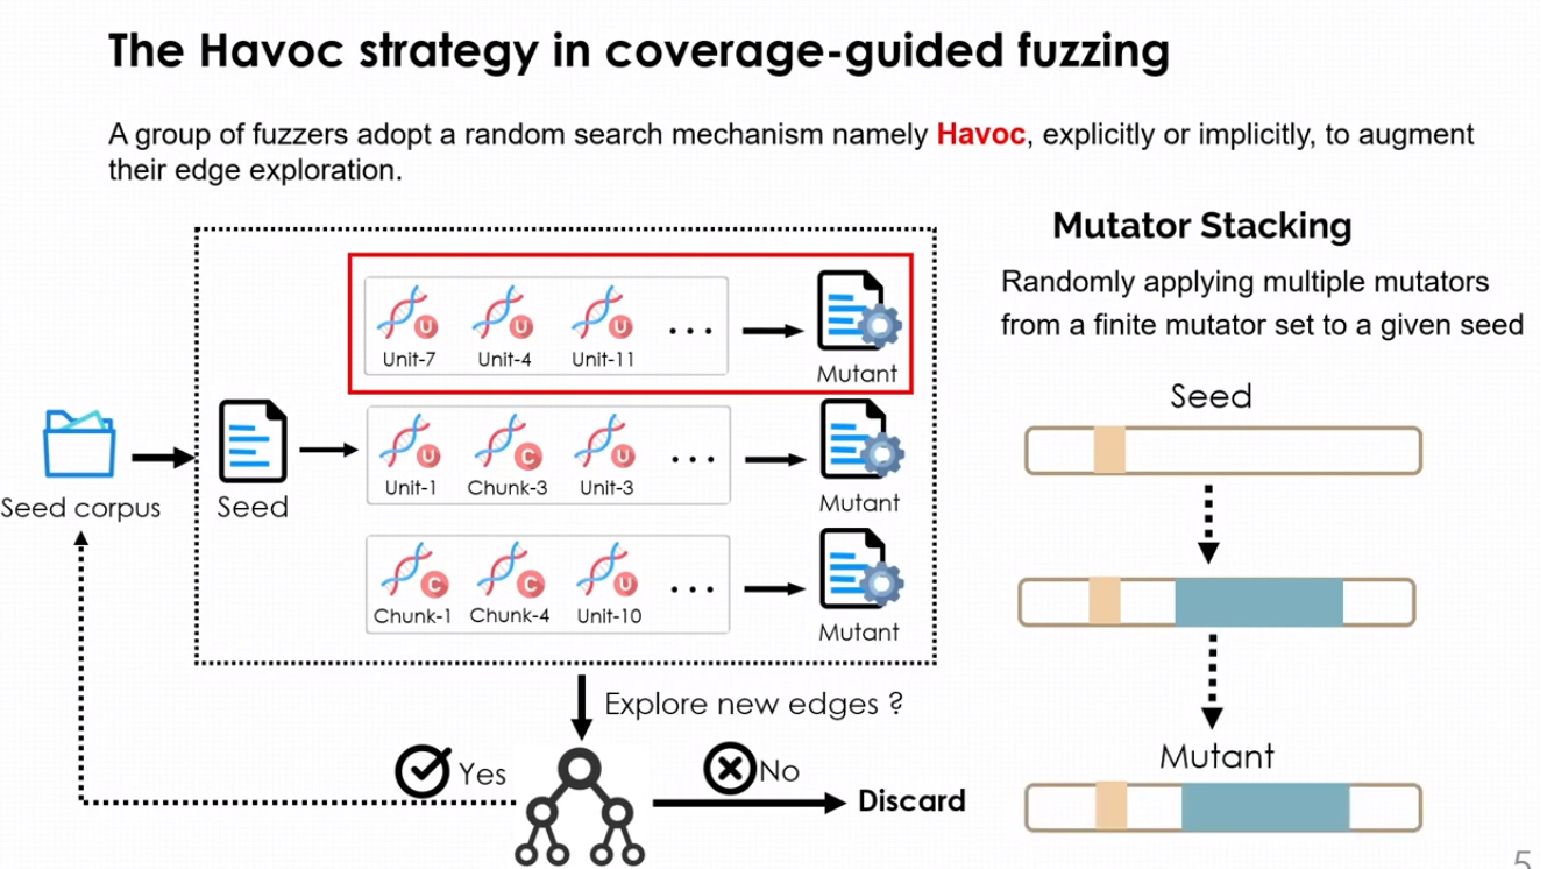
\includegraphics[width=.5\textwidth]{havoc.png}
    \end{center}
    \caption{传统模糊测试}
    \end{figure}
    
    
\end{frame}

\begin{frame}[c]
    {看起来高端但其实}
    \begin{figure}
    \begin{center}
        
\includegraphics[width=.5\textwidth]{zhihu.png}
    \end{center}
    \caption{知乎经典问题}
    \end{figure}
    
\end{frame}

\section{差分测试}
\begin{frame}[c]
    {差分测试}
    \begin{figure}
    \begin{center}
        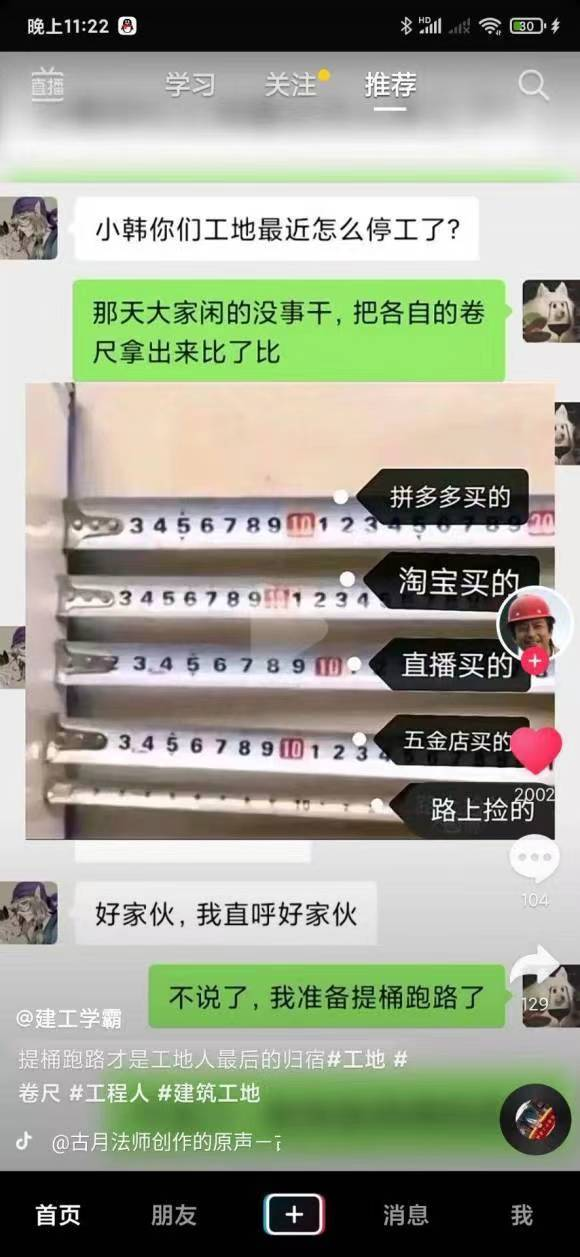
\includegraphics[width=.2\textwidth]{differential.jpeg}
    \end{center}
    \caption{提桶跑路}
    \end{figure}
\end{frame}

\begin{frame}[c]
    {面向编译器的差分测试}
    \begin{figure}
    \begin{center}
        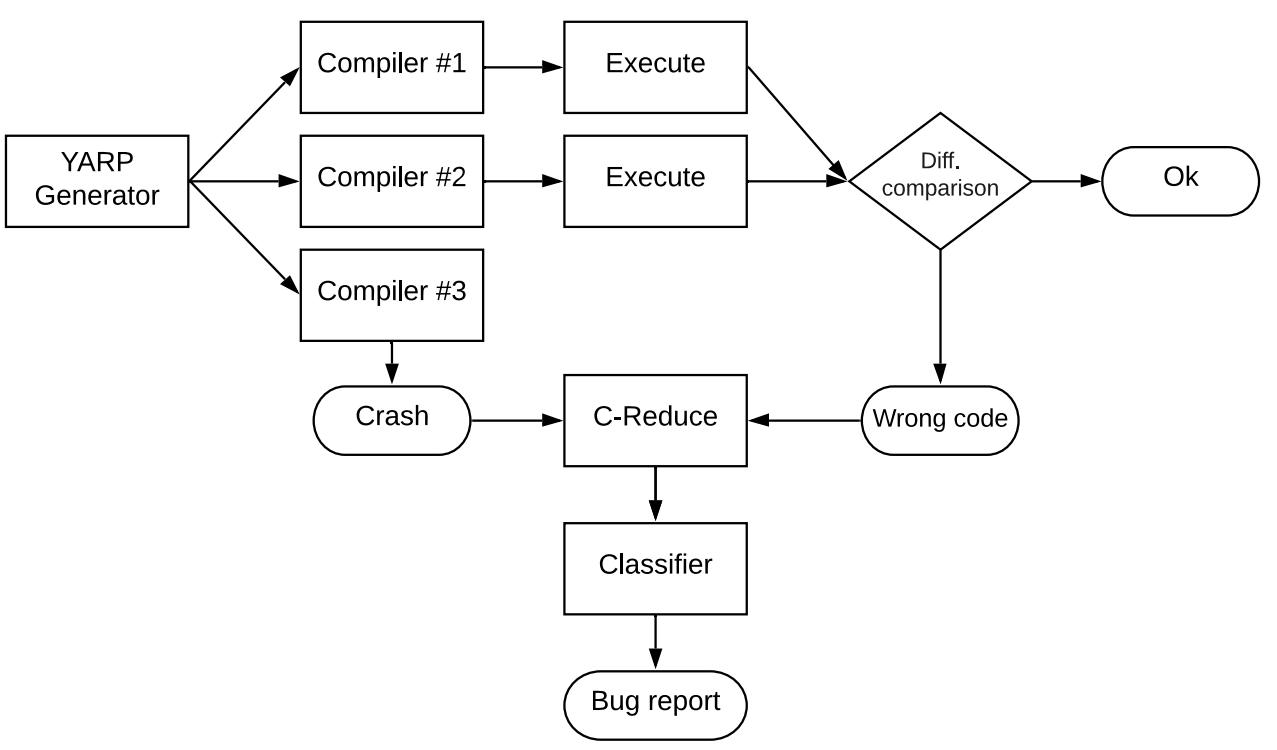
\includegraphics[width=.4\textwidth]{yarpgen.png}
    \end{center}
    \caption{工作流程}
    \end{figure}
    
    
\end{frame}

\section{CSmith}

\begin{frame}{Csmith 原理示意（随机生成 + 类型安全）}

\begin{itemize}
  \item \textbf{Csmith}: 自动生成合法 C 程序，用于编译器测试
  \item \textbf{核心原理}：
  \begin{enumerate}
    \item 随机控制流与表达式生成（if, for, while, switch, 运算符）
    \item 状态跟踪 \& 类型安全保证（变量初始化、数组/指针访问检查）
    \item 输出 C 代码文本，可通过随机种子重复生成
  \end{enumerate}
\end{itemize}

\vspace{0.5cm}
\centering
\begin{tikzpicture}[node distance=0.5cm, >=Stealth, font=\tiny]
  % 节点
  \node[draw, rectangle, fill=blue!20] (seed) {随机种子};
  \node[draw, rectangle, fill=green!20, below=of seed] (flow) {随机控制流生成};
  \node[draw, rectangle, fill=purple!20, below=of flow] (expr) {随机表达式生成};
  \node[draw, rectangle, fill=yellow!20, below=of expr] (state) {状态跟踪 \& 类型安全检查};
  \node[draw, rectangle, fill=orange!20, below=of state] (output) {输出合法 C 程序文本};

  % 箭头
  \draw[->] (seed) -- (flow);
  \draw[->] (flow) -- (expr);
  \draw[->] (expr) -- (state);
  \draw[->] (state) -- (output);

  % 额外说明
  \node[align=center, right=3.5cm of expr] (note) {可控未定义行为\\(防止除零、未初始化使用)};
  \draw[->, dashed] (note.west) -- (state.east);
\end{tikzpicture}

\end{frame}
\begin{frame}[fragile]{BuggyReturnPass}


\begin{lstlisting}
struct BuggyReturnPass : public PassInfoMixin<BuggyReturnPass> {
  PreservedAnalyses run(Module &M, ModuleAnalysisManager &) {
    for (Function &F : M) {
      if (F.isDeclaration()) continue;
      Type *retTy = F.getReturnType();
      // only target integer return types
      if (!retTy->isIntegerTy()) continue;
      IntegerType *IT = cast<IntegerType>(retTy);
      // Build the constant of the *correct* width
      Constant *oneConst = ConstantInt::get(IT, 1);
      for (BasicBlock &BB : F) {
        // iterate carefully since we erase instructions
        for (auto it = BB.begin(); it != BB.end(); ) {
          Instruction &I = *it++;
          if (ReturnInst *RI = dyn_cast<ReturnInst>(&I)) {
            // Insert new return with correct typed constant
            IRBuilder<> B(RI);
            B.CreateRet(oneConst);
            RI->eraseFromParent();
          }
        }
      }
    }
    return PreservedAnalyses::none();
  }
};
\end{lstlisting}

\end{frame}

\begin{frame}[t,fragile]{加载BuggyReturnPass编译}

\begin{verbatim}
$ csmith > a.c
$ clang -O0 -fpass-plugin=./BuggyReturnPass.so a.c \
  -I /usr/include/csmith/ -o a
$ clang a.c -I /usr/include/csmith/ -o b
$ ./a > a.log
$ ./b > b.log
$ diff a.log b.log
1c1
< checksum = BFB85390
---
> checksum = 6B34DC6

\end{verbatim}
\end{frame}

\begin{frame}[t]{探索空间}
    \begin{block}{可考虑的扰动因素}
        \begin{itemize}
            \item 多个编译器
            \item 同一个编译器的多个版本
            \item 同一个编译器的多个优化级别
            \item 等价模输入
        \end{itemize}
    \end{block}
\end{frame}
\begin{frame}[t] {CSmith源码学习}
    \begin{figure}
    \begin{center}
        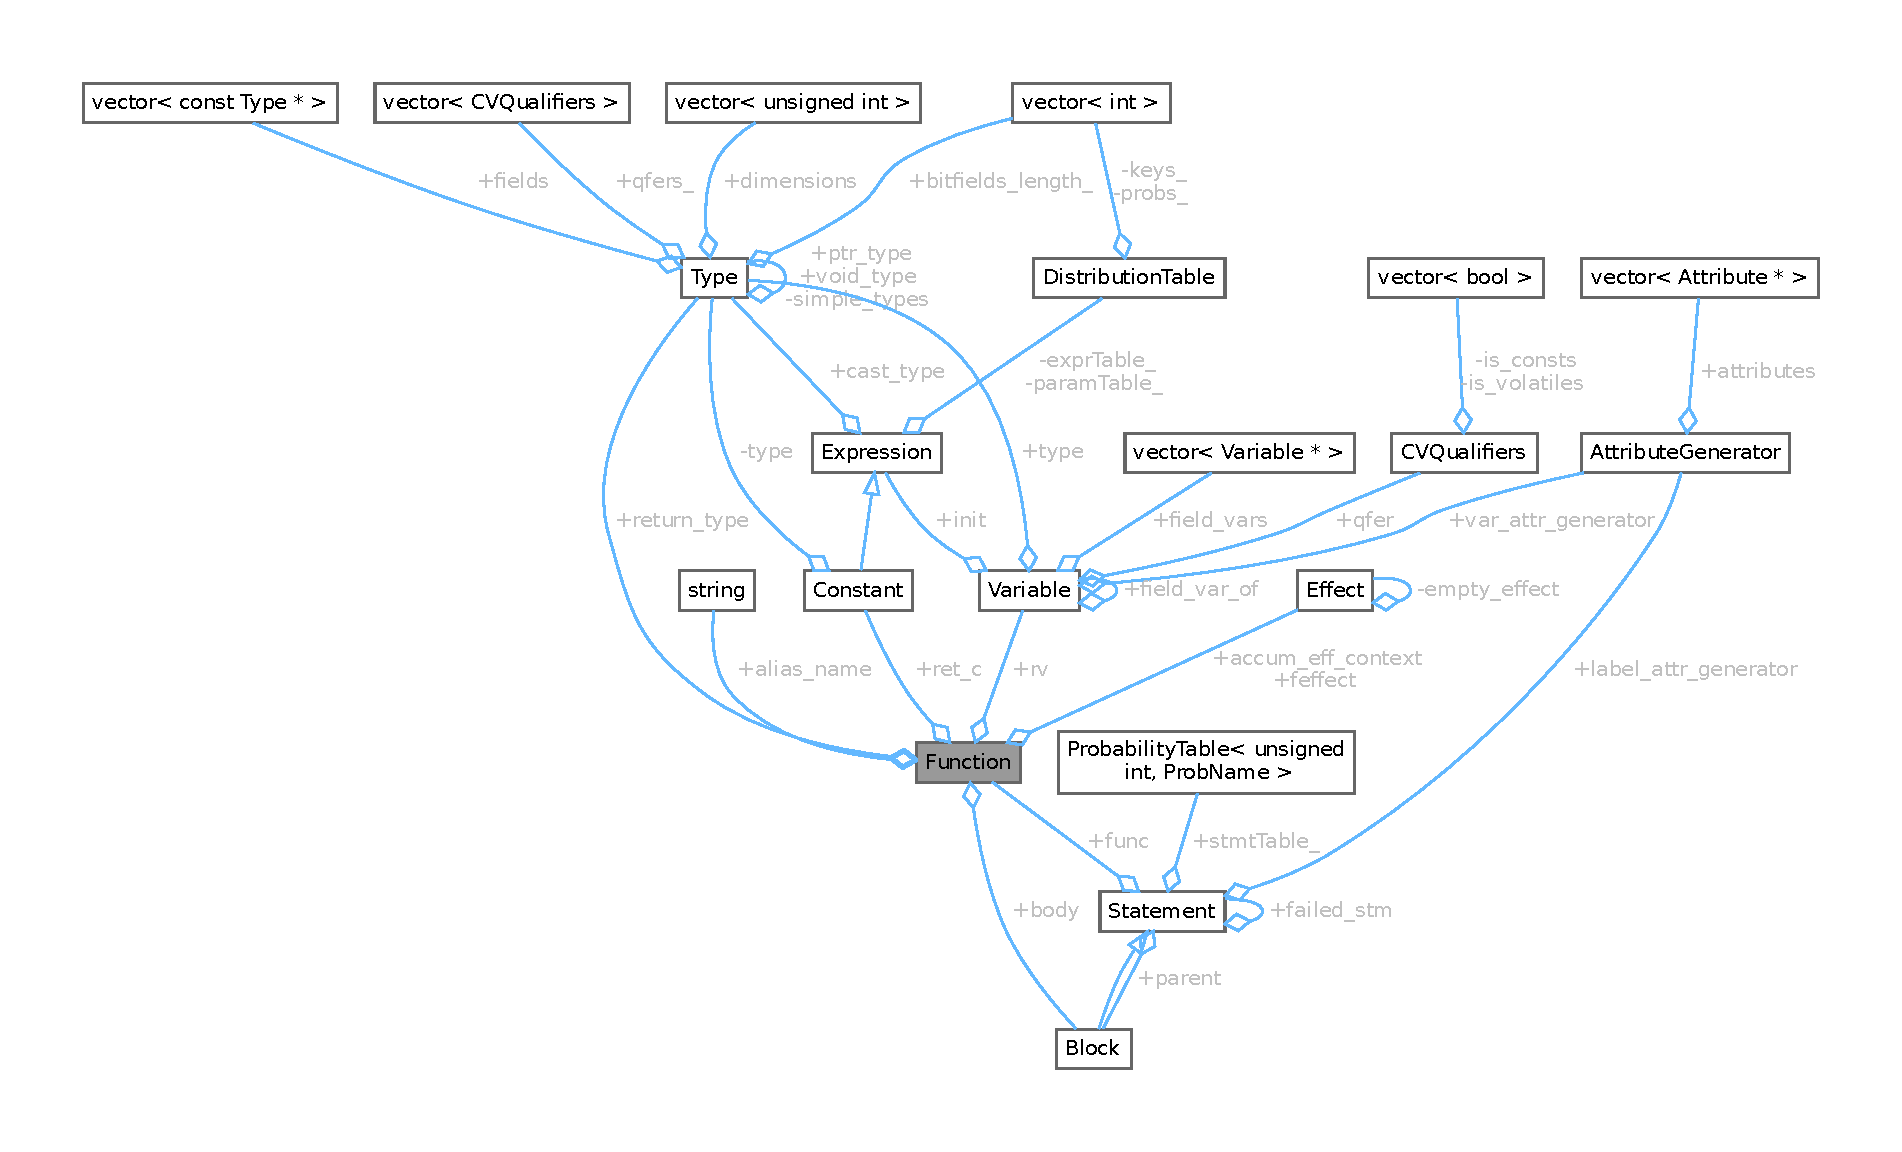
\includegraphics[width=.7\textwidth]{classFunction__coll__graph.dot.pdf}
    \end{center}
    \caption{Function类图}
    \end{figure}
\end{frame}
\begin{frame}[t] {CSmith源码学习}
    \begin{figure}
    \begin{center}
        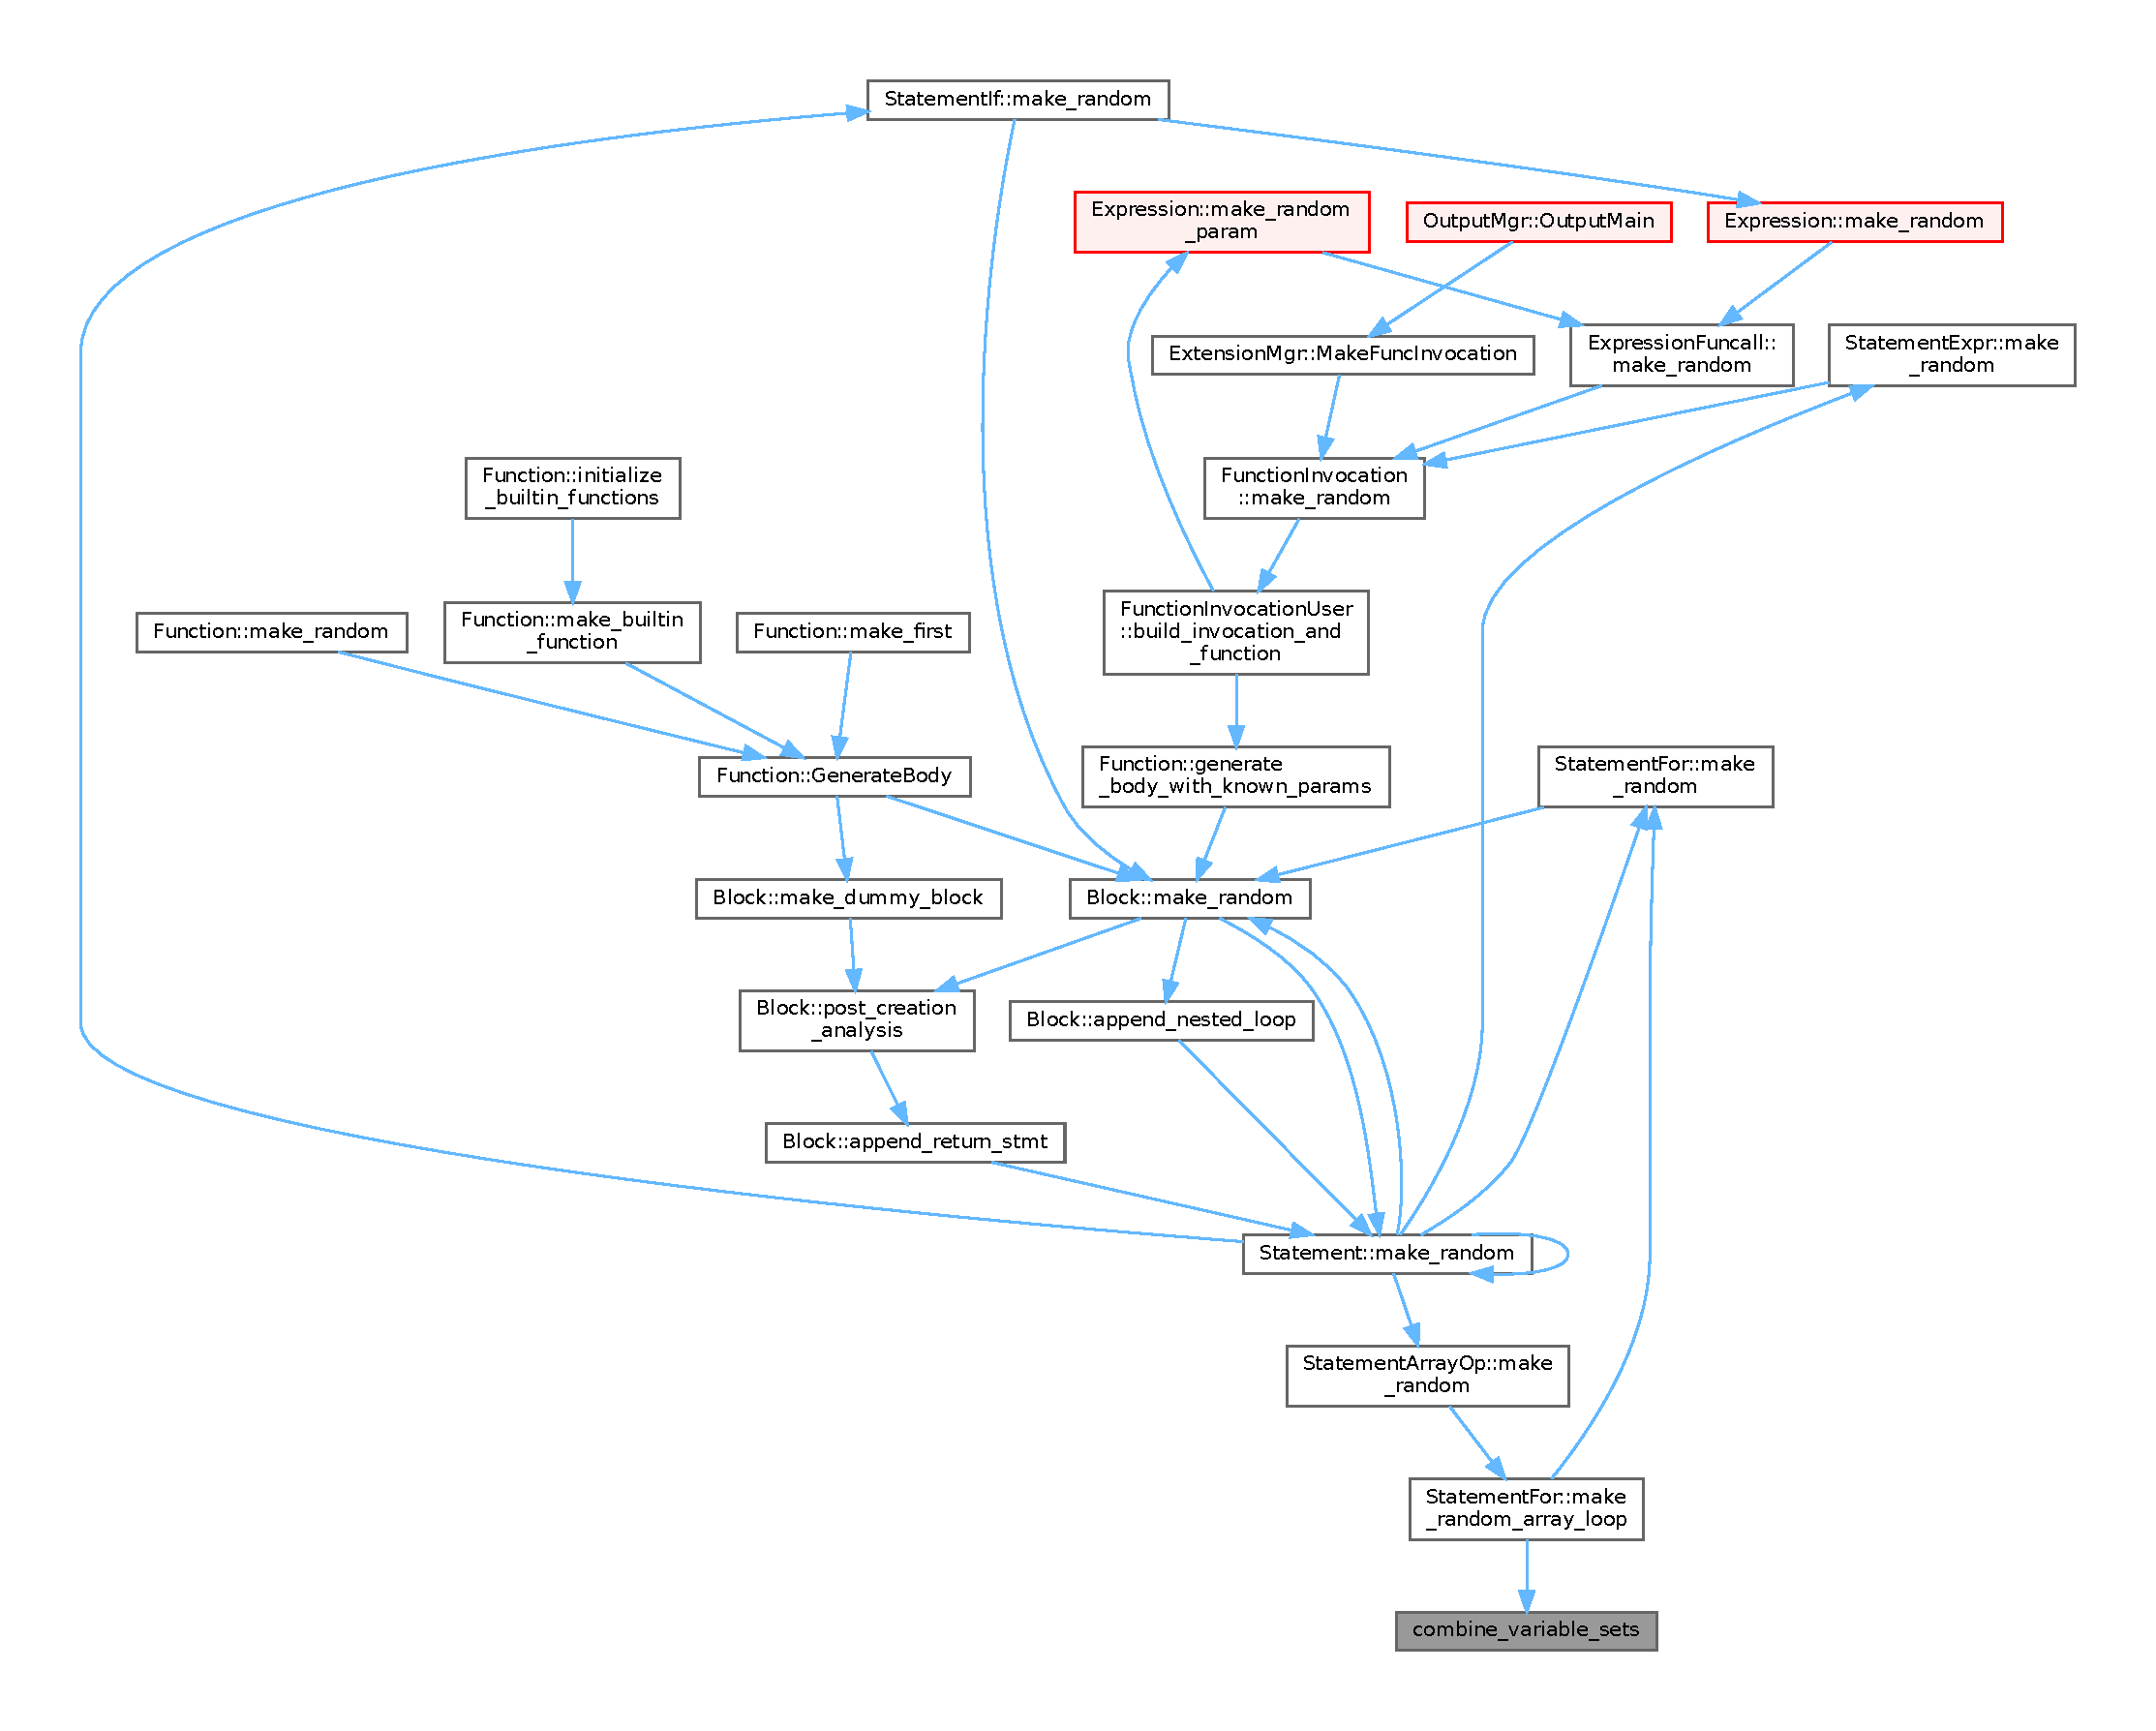
\includegraphics[width=.65\textwidth]{Variable_8cpp_a0a6d19c2f73390302f0bd4e560057e4d_icgraph.dot.pdf}
    \end{center}
    \caption{函数构造调用图}
    \end{figure}
\end{frame}
\end{document}
